\documentclass[12pt, letterpaper]{article}

% --- Packages
\usepackage[utf8]{inputenc}
\usepackage[T1]{fontenc}
\usepackage[margin=2.5cm]{geometry}
\usepackage{makeidx}
\usepackage{natbib}
\usepackage{url}
\usepackage{enumitem}
\usepackage{listings}
\usepackage{xcolor}
\usepackage{parskip}
\usepackage{graphicx}
\usepackage{tikz}
\usepackage[spanish, mexico]{babel}
\usepackage{hyperref} % Enables the creation of hyperlinks
\usepackage{float}

% --- Graphics path
\graphicspath{ {./img/} }

% --- Code format

\definecolor{codegreen}{rgb}{0,0.6,0}
\definecolor{codegray}{rgb}{0.5,0.5,0.5}
\definecolor{codepurple}{rgb}{0.58,0,0.82}
\definecolor{backcolour}{rgb}{0.95,0.95,0.92}

\lstdefinestyle{mystyle}{
	backgroundcolor=\color{backcolour},
	commentstyle=\color{codegreen},
	keywordstyle=\color{magenta},
	numberstyle=\tiny\color{codegray},
	stringstyle=\color{codepurple},
	basicstyle=\ttfamily\footnotesize,
	breakatwhitespace=false,
	breaklines=true,
	captionpos=b,
	keepspaces=true,
	numbers=left,
	numbersep=5pt,
	showspaces=false,
	showstringspaces=false,
	showtabs=false,
	tabsize=2
}

% Allow for some special characters on listings
\lstset{literate=
    {á}{{\'a}}1 {é}{{\'e}}1 {í}{{\'i}}1 {ó}{{\'o}}1 {ú}{{\'u}}1
    {Á}{{\'A}}1 {É}{{\'E}}1 {Í}{{\'I}}1 {Ó}{{\'O}}1 {Ú}{{\'U}}1
    {à}{{\`a}}1 {è}{{\`e}}1 {ì}{{\`i}}1 {ò}{{\`o}}1 {ù}{{\`u}}1
    {À}{{\`A}}1 {È}{{\`E}}1 {Ì}{{\`I}}1 {Ò}{{\`O}}1 {Ù}{{\`U}}1
    {ä}{{\"a}}1 {ë}{{\"e}}1 {ï}{{\"i}}1 {ö}{{\"o}}1 {ü}{{\"u}}1
    {Ä}{{\"A}}1 {Ë}{{\"E}}1 {Ï}{{\"I}}1 {Ö}{{\"O}}1 {Ü}{{\"U}}1
    {â}{{\^a}}1 {ê}{{\^e}}1 {î}{{\^i}}1 {ô}{{\^o}}1 {û}{{\^u}}1
    {Â}{{\^A}}1 {Ê}{{\^E}}1 {Î}{{\^I}}1 {Ô}{{\^O}}1 {Û}{{\^U}}1
    {ã}{{\~a}}1 {ẽ}{{\~e}}1 {ĩ}{{\~i}}1 {õ}{{\~o}}1 {ũ}{{\~u}}1
    {Ã}{{\~A}}1 {Ẽ}{{\~E}}1 {Ĩ}{{\~I}}1 {Õ}{{\~O}}1 {Ũ}{{\~U}}1
    {œ}{{\oe}}1 {Œ}{{\OE}}1 {æ}{{\ae}}1 {Æ}{{\AE}}1 {ß}{{\ss}}1
    {ű}{{\H{u}}}1 {Ű}{{\H{U}}}1 {ő}{{\H{o}}}1 {Ő}{{\H{O}}}1
    {ç}{{\c c}}1 {Ç}{{\c C}}1 {ø}{{\o}}1 {Ø}{{\O}}1 {å}{{\r a}}1 {Å}{{\r A}}1
    {€}{{\euro}}1 {£}{{\pounds}}1 {«}{{\guillemotleft}}1
    {»}{{\guillemotright}}1 {ñ}{{\~n}}1 {Ñ}{{\~N}}1 {¿}{{?`}}1 {¡}{{!`}}1 
}

\lstset{style=mystyle}

% --- Bibliography format
\newlist{biblio}{enumerate}{1}
\setlist[biblio,1]{label=[\arabic*]}

% --- Index
\makeindex

% --- Data

\begin{document}

	\begin{titlepage}
		\begin{center}
			\vspace*{1cm}

			\Huge
			\textbf{Embinux}

			\vspace{0.5cm}
			\Large
			Proceso de creación de un sistema Linux embebido

			Sistemas Operativos\\
			Grupo 6

			
\includegraphics[width=0.5\textwidth]{ingenieria}

			\Large
			Calderón Olalde Enrique Job\\
			Ugartechea Gonzalez Luis Antonio\\
			\textbf{Facultad de Ingeniería}\\
            \today
		\end{center}
	\end{titlepage}

	\section{Introducción}

	\subsection{¿Qué es Linux?}

	Linux es un kernel que en unión con GNU se vuelve un sistema operativo FOSS (Free and Open Source Software) basado en UNIX. El kernel fue creado por Linus Torvalds en 1991. Las herramientas GNU fueron creadas por Richard Stallman en 1983. GNU/Linux es el nombre correcto para referirse a la unión de ambos, aunque comúnmente se le llama Linux a todo el sistema operativo.

	\subsection{¿Qué es un sistema embebido?}

	Un sistema embebido es un sistema informático compuesto por una combinación de hardware y software diseñado para realizar una función específica. Se utilizan actualmente para controlar funciones dentro de un sistema multifunción más grande, tienden a ser de bajo consumo de energía, de bajo costo y de tamaño reducido, facilitando la adaptación para otros dispositivos.

	\subsubsection{Componentes}

	A grandes rasgos, un sistema embebido se compone por lo siguiente:

	\begin{itemize}
		\item \textbf{Microprocesador:} Este componente actúa como el núcleo del sistema, diseñado para tareas específicas. Puede ejecutar instrucciones, controla operaciones y gestionar los recursos del sistema.
		\item \textbf{Memoria:} Hay dos tipos de memoria en un sistema embebido, la memoria RAM (Random Access Memory) para almacenar datos temporales y variables de trabajo. La memoria flash, por otro lado, almacena los datos permanentes del sistema, como el firmware y el sistema operativo, incluyendo la configuración del sistema.
		\item \textbf{Software:} Es la parte ``inteligente'' del sistema, contiene las instrucciones que el sistema ejecuta,encargado del comportamiento y respuestas del mismo.
		\item \textbf{Periféricos:} Estos permiten la interacción del sistema embebido con el exterior. Pueden incluir sensores, actuadores, pantallas, teclados, entre otros.
	\end{itemize}

	\subsection{Linux en sistemas embebidos}

	Linux se ha convertido en una opción muy popular para sistemas embebidos debido a su flexibilidad, escalabilidad, estabilidad y por ser open source. Su arquitectura modular permite adaptar el sistema operativo a las necesidades específicas del dispositivo, eliminando componentes innecesarios para ahorrar espacio y recursos.

	\subsection{Ventajas de Linux embebido}

	Una de las principales ventajas de utilizar Linux en sistemas embebidos es el acceso a una gran comunidad y a una amplia gama de herramientas y bibliotecas. Facilitando el desarrollo y mantenimiento. Además, existen versiones específicas de Linux diseñadas para sistemas con recursos limitados, como \textit{Yocto}, \textit{Buildroot}, \textit{OpenWrt}, etc.

	En este contexto, el kernel Linux puede ser configurado para soportar únicamente el hardware del sistema embebido en cuestión, reduciendo el tiempo de arranque y el uso de memoria. También es posible integrar controladores específicos y definir mecanismos de comunicación eficientes con los periféricos del dispositivo.

	\subsection{Casos comunes de uso}

	El uso de Linux en sistemas embebidos abarca una gran variedad de industrias y dispositivos. Algunos de los casos más comunes:

	\begin{itemize}
		\item \textbf{Routers y dispositivos de red:} Linux es ampliamente utilizado en enrutadores domésticos y comerciales, switches y firewalls. %Distribuciones como OpenWrt y DD-WRT permiten a los fabricantes y usuarios personalizar el comportamiento de sus dispositivos, optimizar el rendimiento de la red, e incorporar funcionalidades como VPNs, QoS, y servidores integrados.

		\item \textbf{Televisores inteligentes y set-top boxes:} Muchos Smart TVs y dispositivos de streaming en el mercado utilizan Linux como sistema operativo base, debido a su capacidad de ejecutar interfaces gráficas, manejar decodificación multimedia y permitir actualizaciones OTA (Over-The-Air). % Plataformas como Android TV, que se basa en el kernel de Linux, dominan este mercado.

		\item \textbf{Automatización industrial:} En entornos industriales, Linux embebido se emplea en controladores lógicos programables (PLCs), sistemas SCADA, paneles HMI (Human-Machine Interface), etc. % Su estabilidad y soporte para redes industriales como Modbus o CANbus lo hacen ideal para tareas críticas.

		\item \textbf{Electrodomésticos inteligentes:} En refrigeradores, lavadoras, hornos, aspiradoras robot y otros dispositivos del hogar inteligente utilizan Linux embebido para conectividad, control remoto, programación de tareas, y comunicación con asistentes de voz. % Su compatibilidad con protocolos como MQTT y Zigbee facilita su integración al ecosistema del IoT.

		\item \textbf{Automóviles:} Muchas unidades de control electrónico (ECUs) y sistemas de infoentretenimiento en automóviles modernos utilizan Linux embebido. % Iniciativas como Automotive Grade Linux (AGL) promueven una plataforma común y estandarizada para fabricantes automotrices, permitiendo reducir costos y acelerar el desarrollo de software.

		\item \textbf{Dispositivos portátiles y wearables:} Relojes inteligentes, rastreadores de actividad, cámaras deportivas y dispositivos GPS también hacen uso de Linux debido a su bajo consumo energético % Permiten compatibilidad con Bluetooth y sensores, y capacidad para ejecutar interfaces de usuario eficientes en pantallas pequeñas.
	\end{itemize}

	Estas aplicaciones son algunas de las más utilizadas aunque también se encuentra presente en otros dispositivos como cámaras de seguridad, drones, sistemas de control de acceso, sistemas de monitoreo ambiental, entre otros.

	% \section{Componentes}

	% \subsection{Kernel}

	% El \textbf{kernel} es el núcleo de un sistema operativo; actúa como intermediario entre el hardware y el software. Es responsable de gestionar el acceso al procesador, la memoria y los controladores (drivers) más importantes, permitiendo así la comunicación directa con el hardware.

	% Aunque puede variar en complejidad y diseño, un kernel suele estar organizado en varias capas funcionales:

	% \begin{itemize}
	% 	\item \textbf{Interfaz con el hardware:} Es la capa más baja y se encarga de tareas como la gestión de controladores de red, controladores de buses como PCI Express, y otros elementos específicos del hardware.
	% 	\item \textbf{Gestión de memoria:} Asigna y distribuye la memoria entre los procesos, controla el acceso a la memoria física y virtual, y maneja técnicas como la paginación o la segmentación.
	% 	\item \textbf{Gestión de procesos:} Supervisa la creación, ejecución, suspensión y finalización de los procesos, además de encargarse de la planificación (scheduling) y sincronización entre ellos.
	% 	\item \textbf{Gestión de dispositivos:} Controla el acceso a los dispositivos de entrada/salida (E/S), como discos duros, impresoras, teclados, entre otros, a través de sus respectivos controladores.
	% 	\item \textbf{Gestión del sistema de archivos:} Regula el acceso a archivos y directorios, manteniendo la organización lógica de los datos almacenados y garantizando su integridad.
	% \end{itemize}

	% \subsection{Sistema de archivos}

	% Un sistema de archivos es el componente del sistema operativo encargado de organizar, almacenar y recuperar datos en un medio de almacenamiento, como un disco duro o una memoria flash. Define cómo se estructuran los datos y cómo se accede a ellos.

	% \subsubsection{Componentes principales}

	% \begin{itemize}
	% 	\item \textbf{Estructura de directorios:} Organización jerárquica que permite agrupar archivos en carpetas y subcarpetas.
	% 	\item \textbf{I-nodos (o estructuras de control):} Contienen metadatos de cada archivo, como permisos, tamaño, fechas de creación/modificación y ubicación física en el disco.
	% 	\item \textbf{Bloques de datos:} Espacios del medio de almacenamiento donde se guarda el contenido real de los archivos.
	% 	\item \textbf{Tabla de asignación:} Registra cómo se distribuyen los bloques de datos entre los archivos. Ejemplos incluyen FAT (File Allocation Table) y estructuras similares en otros sistemas.
	% 	\item \textbf{Gestor de permisos:} Controla el acceso a archivos y directorios, definiendo qué usuarios pueden leer, escribir o ejecutar.
	% 	\item \textbf{Journaling:} Mecanismo que registra operaciones pendientes para mantener la integridad del sistema de archivos en caso de fallos o apagados inesperados.
	% \end{itemize}

	\section{Proceso de creación (buildroot)}

	Para crear este sistema embebido, se utilizará Buildroot. Buildroot es una herramienta de construcción de sistemas Linux embebidos que permite crear un sistema Linux completo a partir de un conjunto de paquetes y configuraciones.

	Buildroot utiliza un proceso con cross-compilation para generar un sistema Linux que se puede ejecutar en una arquitectura diferente a la de la computadora de desarrollo. Esto es posible gracias a que Buildroot incluye su propio compilador y herramientas de construcción, lo que facilita la creación de un sistema embebido personalizado.

	\subsection{Herramientas}

	Para compilar un sistema embebido con Buildroot, se requieren las siguientes herramientas y condiciones:

	\begin{itemize}
		\item \textbf{Compilador:} Buildroot puede generar su propio cross-compiler basado en \texttt{gcc},así como seleccionar diferentes bibliotecas estándar de C como \texttt{glibc}, \texttt{uClibc-ng} o \texttt{musl}.
		\item \textbf{Herramientas de construcción:} Buildroot incluye herramientas de construcción como \texttt{make}, \texttt{tar}, \texttt{gzip}, entre otras.
		\item \textbf{Sistema operativo:} Buildroot se puede ejecutar en cualquier sistema operativo Linux.
		\item \textbf{Conexión a internet:} Se necesita una conexión a internet para descargar los paquetes y herramientas necesarias para la construcción del sistema embebido. Esto pues buildroot compila de fuente todos los paquetes necesarios para el sistema embebido.
		\item \textbf{Hardware:} Se necesita una computadora con suficiente capacidad de procesamiento y memoria para compilar el sistema embebido. Esto pues la compilación puede tardar varias horas dependiendo del tamaño del sistema embebido y la velocidad de la computadora.
	\end{itemize}

	\subsection{Selección de hardware}

	Gracias a que buildroot usa su propio compilador, es posible compilar un sistema embebido para cualquier arquitectura. Esto permite usar buildroot para compilar un sistema embebido para una gran variedad de hardware, desde microcontroladores hasta computadoras de escritorio.

	\subsection{Configuración de buildroot}

	Para compilar un sistema embebido con buildroot, es necesario configurar el sistema embebido. Esto incluye seleccionar la arquitectura del hardware, el sistema de archivos, las aplicaciones de usuario y las herramientas necesarias para el sistema embebido.

	Buildroot incluye una interfaz gráfica llamada \texttt{make menuconfig} que permite seleccionar las opciones deseadas para el sistema embebido. Esta interfaz es similar a la de otras herramientas de construcción como la del mismo kernel Linux.

	\subsection{Compilación}

	Una vez que se ha configurado el sistema embebido, se puede iniciar la compilación. Esto se hace usando el comando \texttt{make}. Este comando iniciará la compilación del sistema embebido y generará una imagen de disco que se puede usar para instalar el sistema en el hardware seleccionado.

	\subsection{Instalación}

	Una vez que la compilación ha finalizado, se generará una imagen de disco que se puede usar para instalar el sistema embebido en el hardware seleccionado. La configuración de la imagen de disco dependerá del hardware seleccionado.

	\section{Ejemplo práctico}

	Para este ejemplo decidimos usar una Raspberry Pi 4 de 4GB, esto pues es una tarjeta común en el mercado además de que gracias a su tamaño puede ser usada en una gran variedad de proyectos.

	El objetivo de este ejemplo práctico es mostrar el uso mínimo de recursos que se puede lograr al compilar un sistema embebido. Para esto, se usará buildroot para compilar un sistema Linux embebido para la Raspberry Pi 4. El sistema embebido tendrá unicamente un entorno de términal y para efectos educativos contará con su instalación de python junto al editor de texto vim.

	En esta ocasión nos comunicaremos con el sistema embebido utilizando la conexión serial de la Raspberry Pi 4. Para esto, se usará un adaptador USB a serial TTL. Con esto evitaremos usar un monitor y teclado además de conexión a red.

	\subsection{Hardware}

	La tarjeta es una computadora que incluye un procesador ARM Cortex-A72, 4GB de RAM y soporte para HDMI, USB y Ethernet. La Raspberry Pi 4 es una Single Board Computer (SBC) por lo que todo el hardware se contiene en una sola tarjeta.

	\subsection{Configuración de buildroot}

	Para la configuración de buildroot se inicia con un clon del repositorio de buildroot:

	\begin{lstlisting}[language=bash]
		git clone https://github.com/buildroot/buildroot.git
	\end{lstlisting}

	Considerando que la Raspberry Pi 4 es una SBC muy común, podemos partir de una configuración ya hecha para esta tarjeta. Para esto, se puede usar el comando \texttt{make} seguido del nombre de la configuración deseada. En este caso, la configuración es \texttt{make raspberrypi4\_64\_defconfig}.

	\begin{lstlisting}[language=bash]
		make raspberrypi4_64_defconfig
	\end{lstlisting}

	Esto generará un archivo de configuración en \texttt{.config} que contiene todas las opciones necesarias para compilar el sistema embebido.

	\subsection{Configuración de herramientas}

	Para configurar nuestro sistema más allá de lo que se encuentra en la configuración por defecto, se puede usar el comando \texttt{make menuconfig}. Este comando abrirá una interfaz gráfica en la terminal que permite seleccionar las opciones deseadas.

	\begin{figure}[H]
		\centering
		\begin{center}
			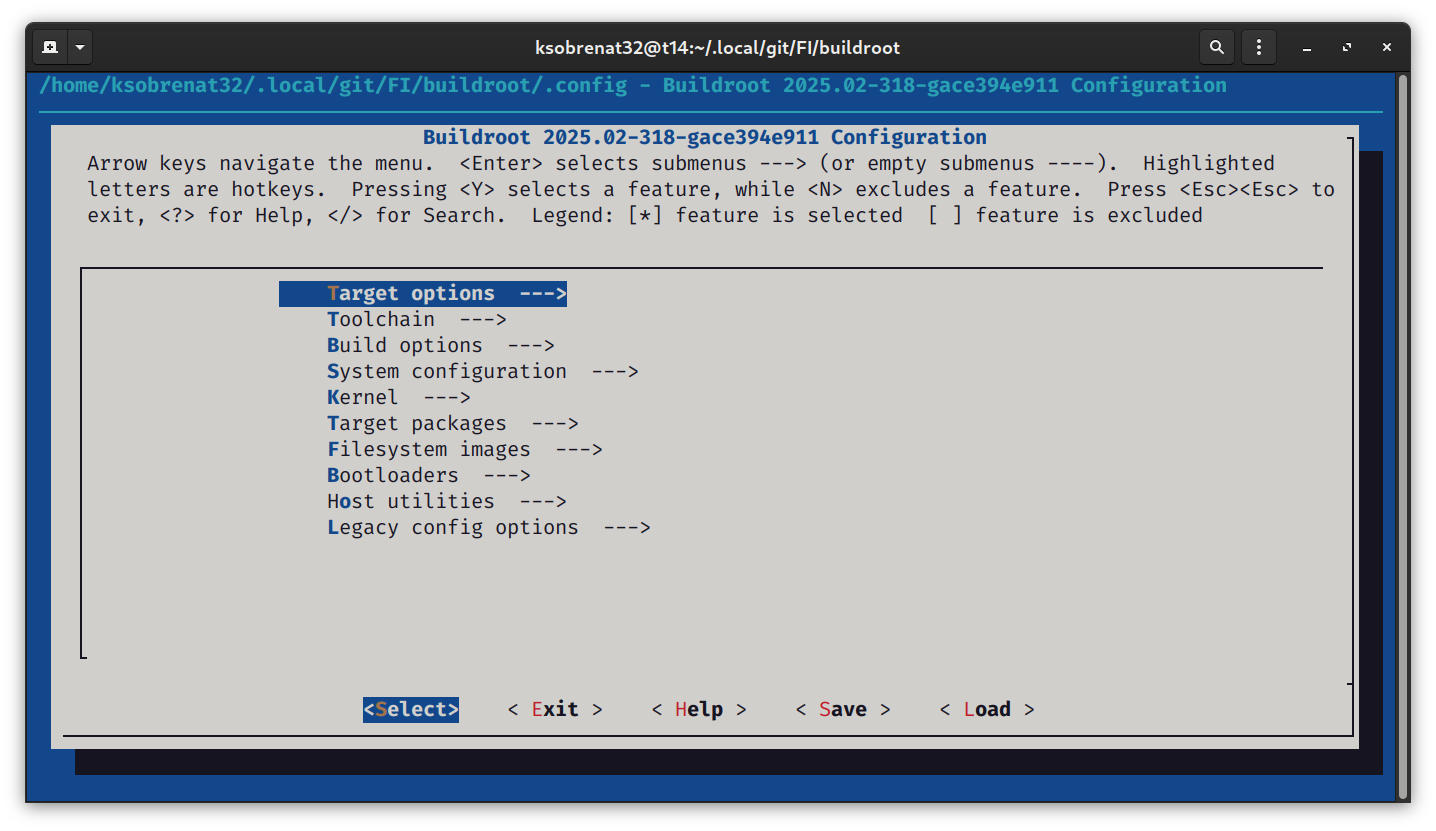
\includegraphics[width=\textwidth]{img/make-menuconfig-01}
			\caption{Interfaz gráfica de \texttt{make menuconfig}}
			\label{fig:make-menuconfig-01}
		\end{center}
	\end{figure}

	Para reducir el tamaño del sistema embebido, Se seleccionará \texttt{musl} en lugar de \texttt{glibc} como la biblioteca estándar de C. Esto permitirá reducir aún el tamaño del sistema embebido.

	\begin{figure}[H]
		\centering
		\begin{center}
			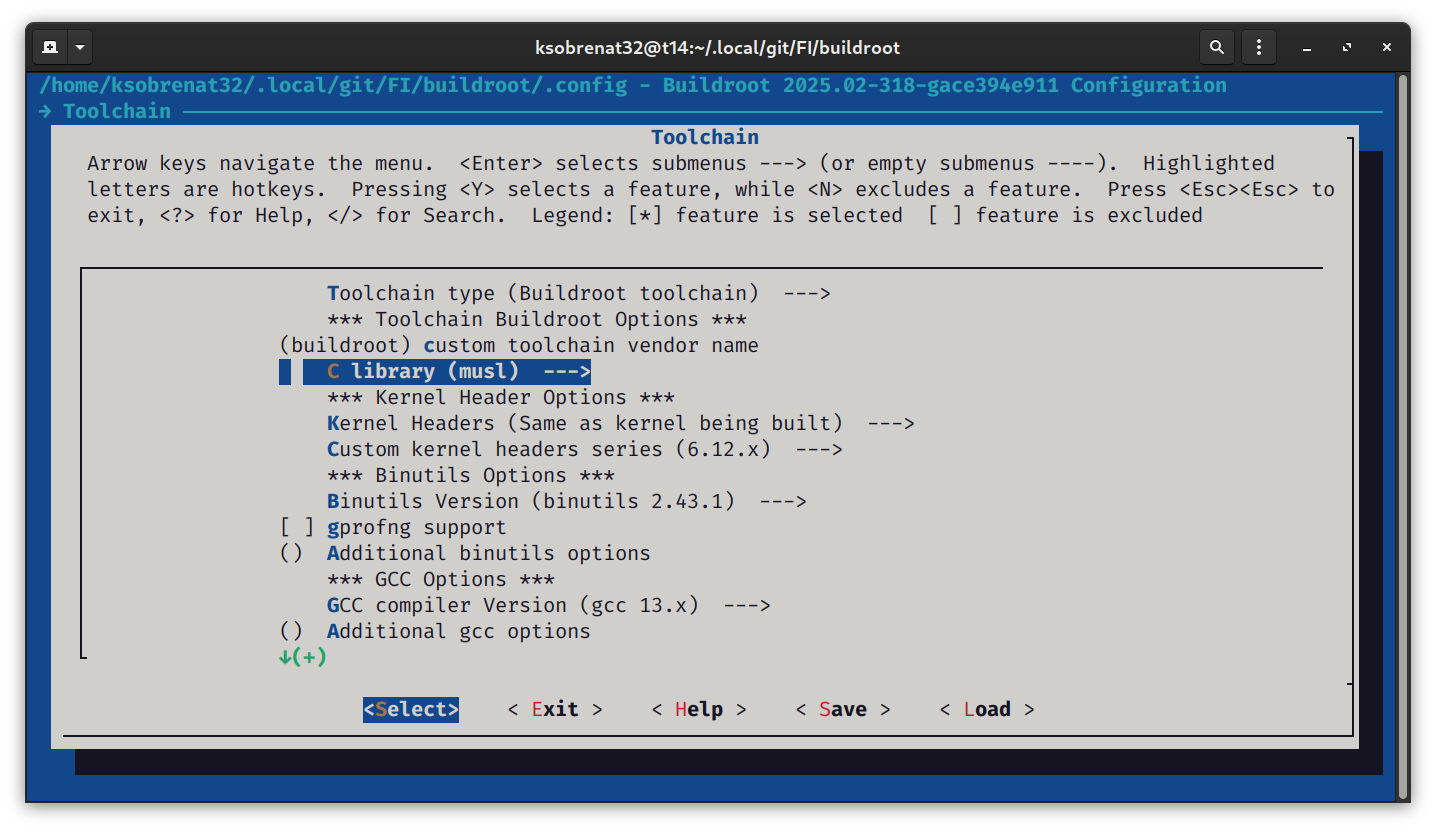
\includegraphics[width=\textwidth]{img/make-menuconfig-02}
			\caption{Configuración de \texttt{musl} como biblioteca estándar de C}
			\label{fig:make-menuconfig-02}
		\end{center}
	\end{figure}

	En cuanto a las aplicaciones de usuario, se seleccionará \texttt{vim} como editor de texto y \texttt{python3} como intérprete de python. Esto permitirá tener un entorno de desarrollo básico en el sistema embebido.

	\begin{figure}[H]
		\centering
		\begin{center}
			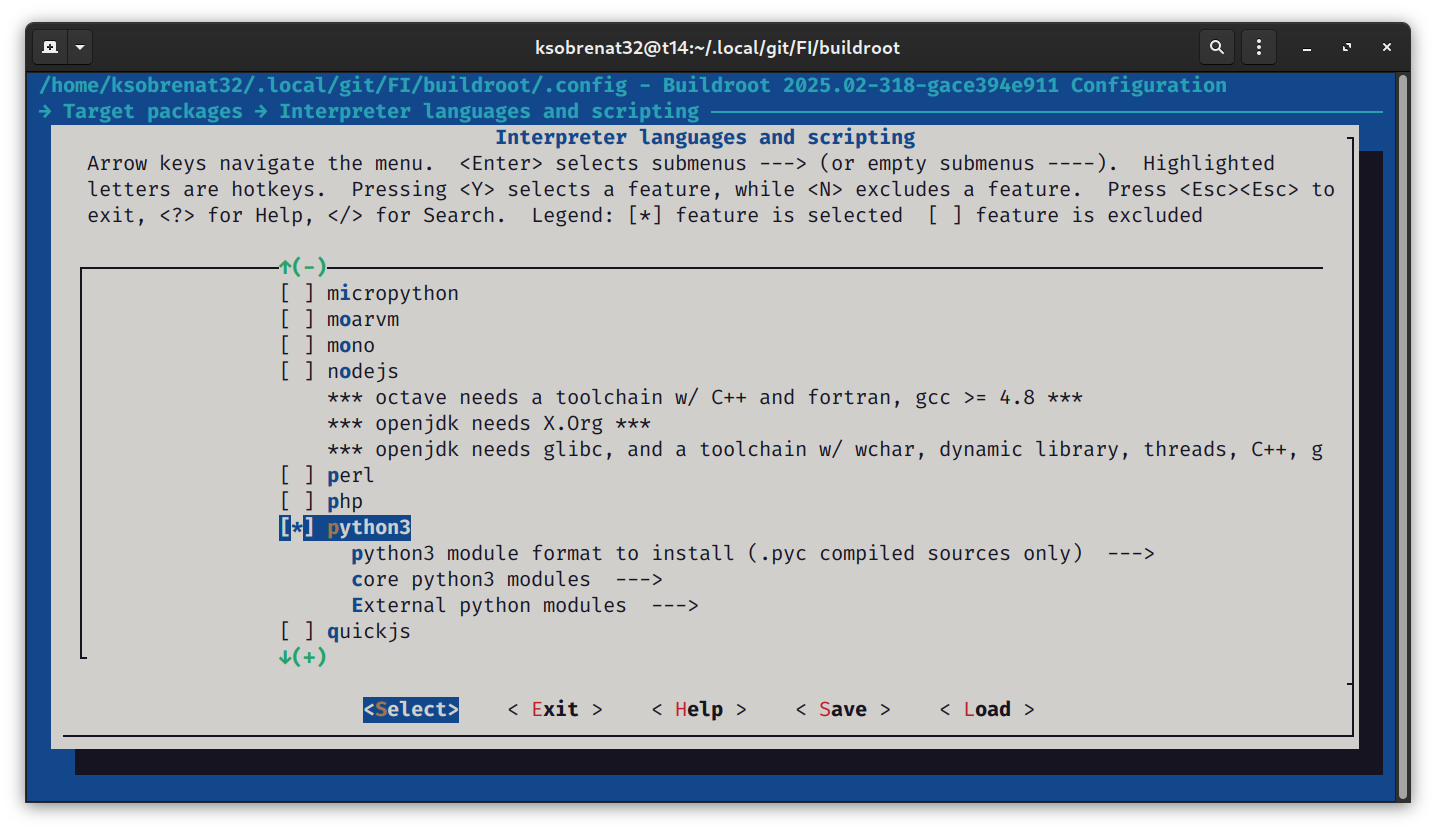
\includegraphics[width=\textwidth]{img/make-menuconfig-03}
			\caption{Instalación de \texttt{python3}}
			\label{fig:make-menuconfig-03}
		\end{center}
	\end{figure}

	\begin{figure}[H]
		\centering
		\begin{center}
			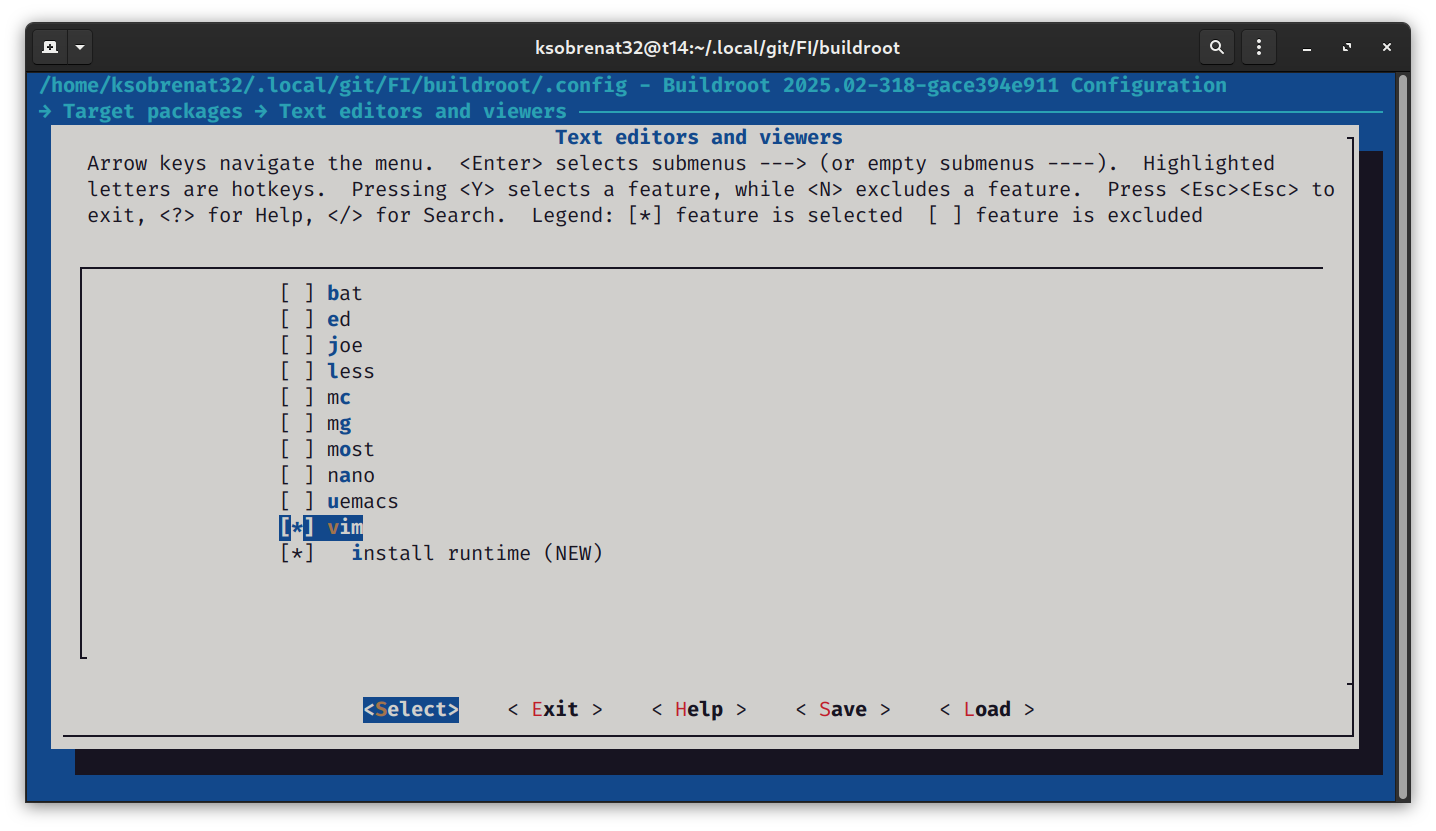
\includegraphics[width=\textwidth]{img/make-menuconfig-04}
			\caption{Instalación de \texttt{vim}}
			\label{fig:make-menuconfig-04}
		\end{center}
	\end{figure}

	Añadiremos htop como herramienta de monitoreo del sistema. Esto permitirá ver el uso de CPU, memoria y procesos en ejecución.

	\begin{figure}[H]
		\centering
		\begin{center}
			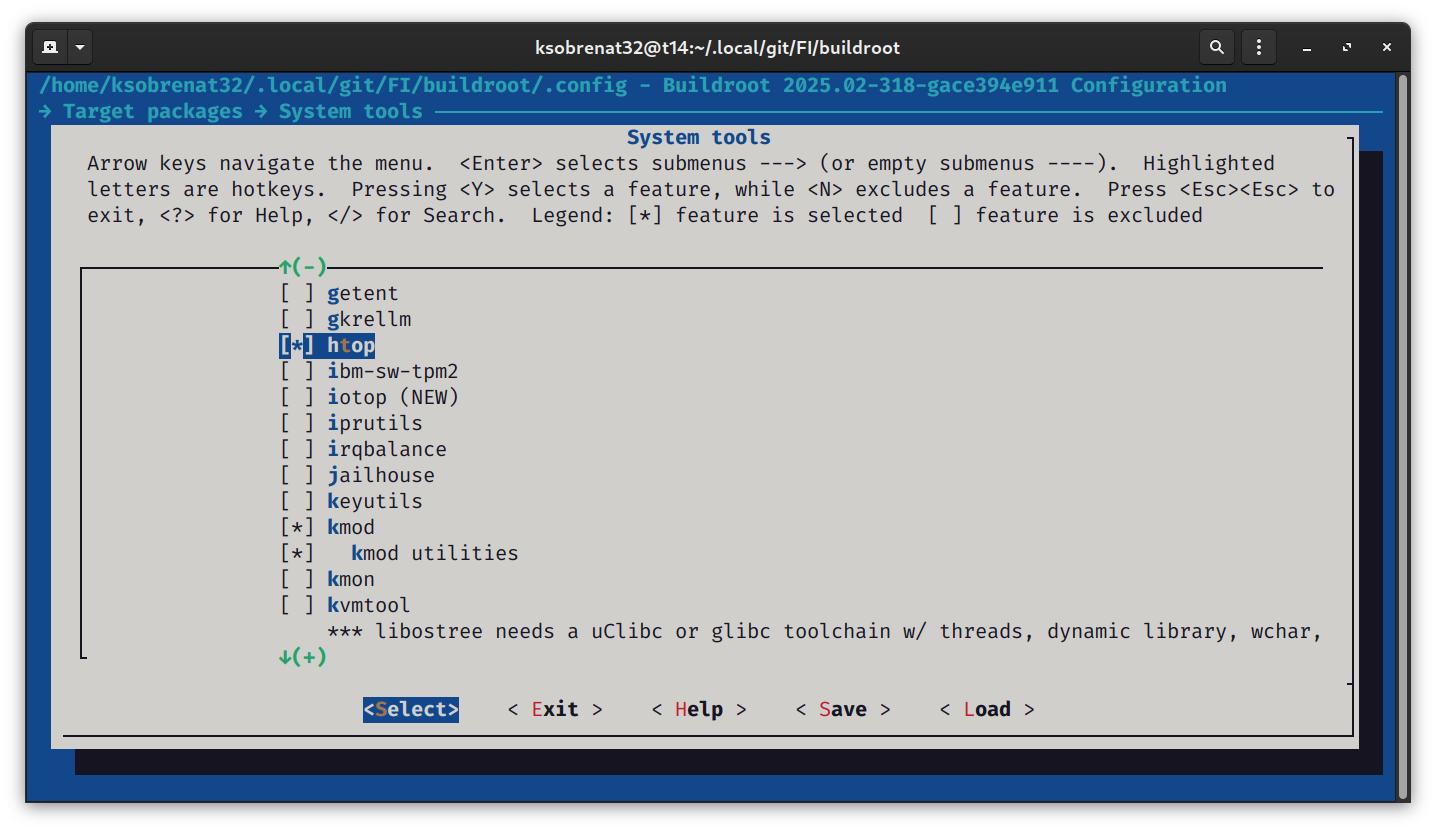
\includegraphics[width=\textwidth]{img/make-menuconfig-05}
			\caption{Instalación de \texttt{htop}}
			\label{fig:make-menuconfig-05}
		\end{center}
	\end{figure}

	Con esto, se ha configurado el sistema embebido para que tenga un entorno de terminal básico con python y vim. Se puede agregar más software si se desea, pero esto aumentará el tamaño del sistema embebido.

	\subsection{Compilación}

	Para empezar la compilación del sistema embebido, se usa el comando \texttt{make}. Este comando iniciará la compilación del sistema embebido y generará una imagen de disco que se puede usar para instalar el sistema en la tarjeta Raspberry Pi 4.

	A diferencia de otras herramientas, buildroot no requiere de un compilador externo. Buildroot incluye su propio compilador y herramientas de construcción, lo que facilita la creación de un sistema embebido personalizado. Además, podemos olvidarnos de indicar el número de núcleos de la computadora, ya que buildroot se encarga de esto automáticamente.

	\begin{figure}[H]
		\centering
		\begin{center}
			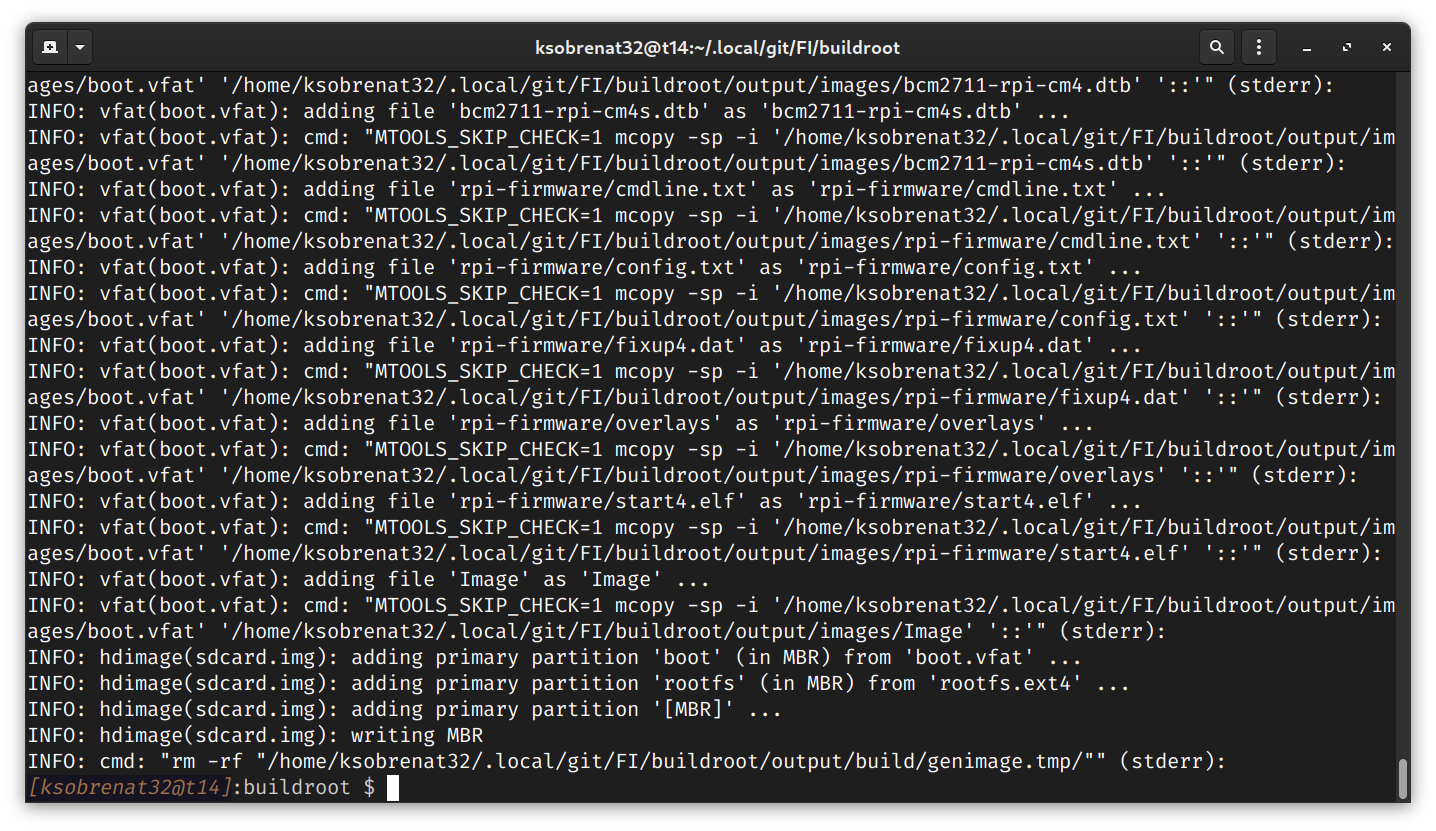
\includegraphics[width=\textwidth]{img/make-compile}
			\caption{Compilación finalizada con éxito}
			\label{fig:make-compile}
		\end{center}
	\end{figure}

	\subsection{Instalación}

	Una vez que la compilación ha finalizado, se generará una imagen de disco en la carpeta \texttt{output/images}. Esta imagen se puede usar para instalar el sistema embebido en la tarjeta Raspberry Pi 4.

	Para instalar el sistema embebido en la tarjeta, se puede usar el comando \texttt{dd} para copiar la imagen de disco a la tarjeta SD. Asegúrate de que la tarjeta SD esté conectada a la computadora y que sepas cuál es el dispositivo correspondiente (por ejemplo, /dev/sdX).

	\begin{lstlisting}[language=bash]
		sudo dd if=output/images/sdcard.img of=/dev/sdX bs=4M status=progress
		sync
	\end{lstlisting}

	\subsection{Pruebas}

	Una vez que la imagen ha sido copiada a la tarjeta SD, se puede insertar la tarjeta en la Raspberry Pi 4 y encenderla. El sistema embebido debería arrancar y mostrar un entorno de terminal.

	\begin{figure}[H]
		\centering
		\begin{center}
			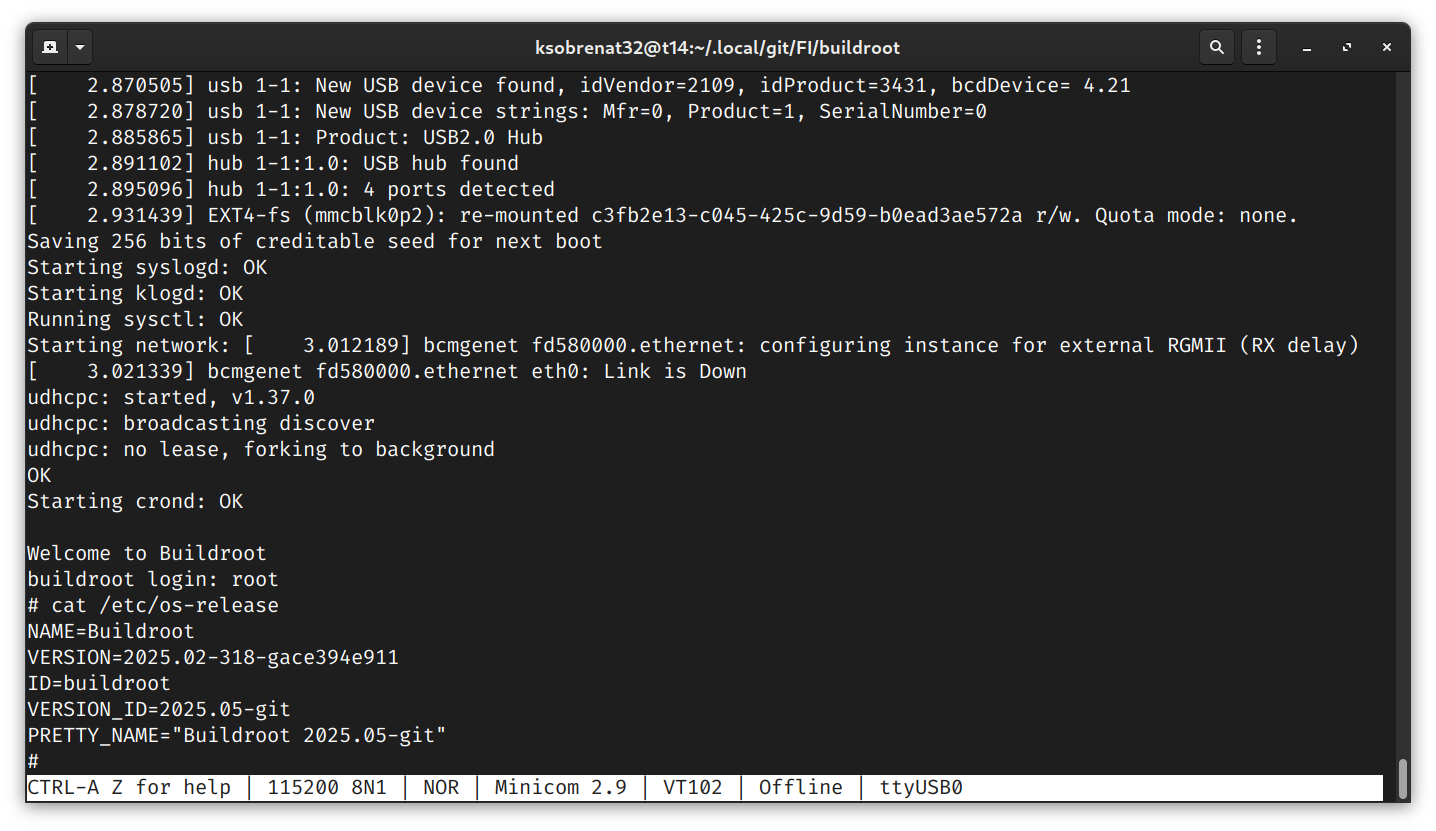
\includegraphics[width=\textwidth]{img/run-example-01}
			\caption{Arranque del sistema embebido}
			\label{fig:boot}
		\end{center}
	\end{figure}


	\begin{figure}[H]
		\centering
		\begin{center}
			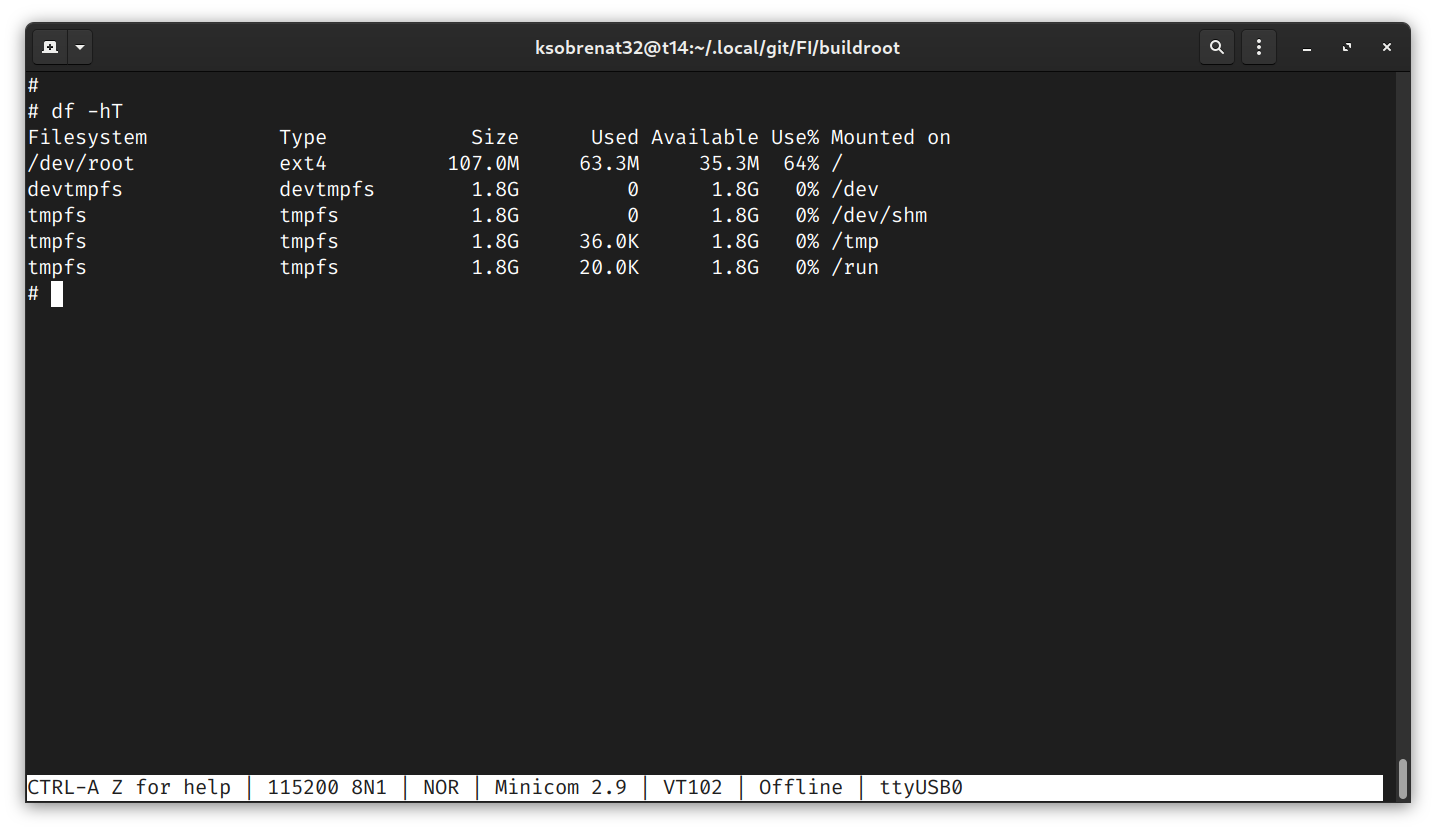
\includegraphics[width=\textwidth]{img/run-example-02}
			\caption{Uso del sistema de archivos}
			\label{fig:boot}
		\end{center}
	\end{figure}

	\begin{figure}[H]
		\centering
		\begin{center}
			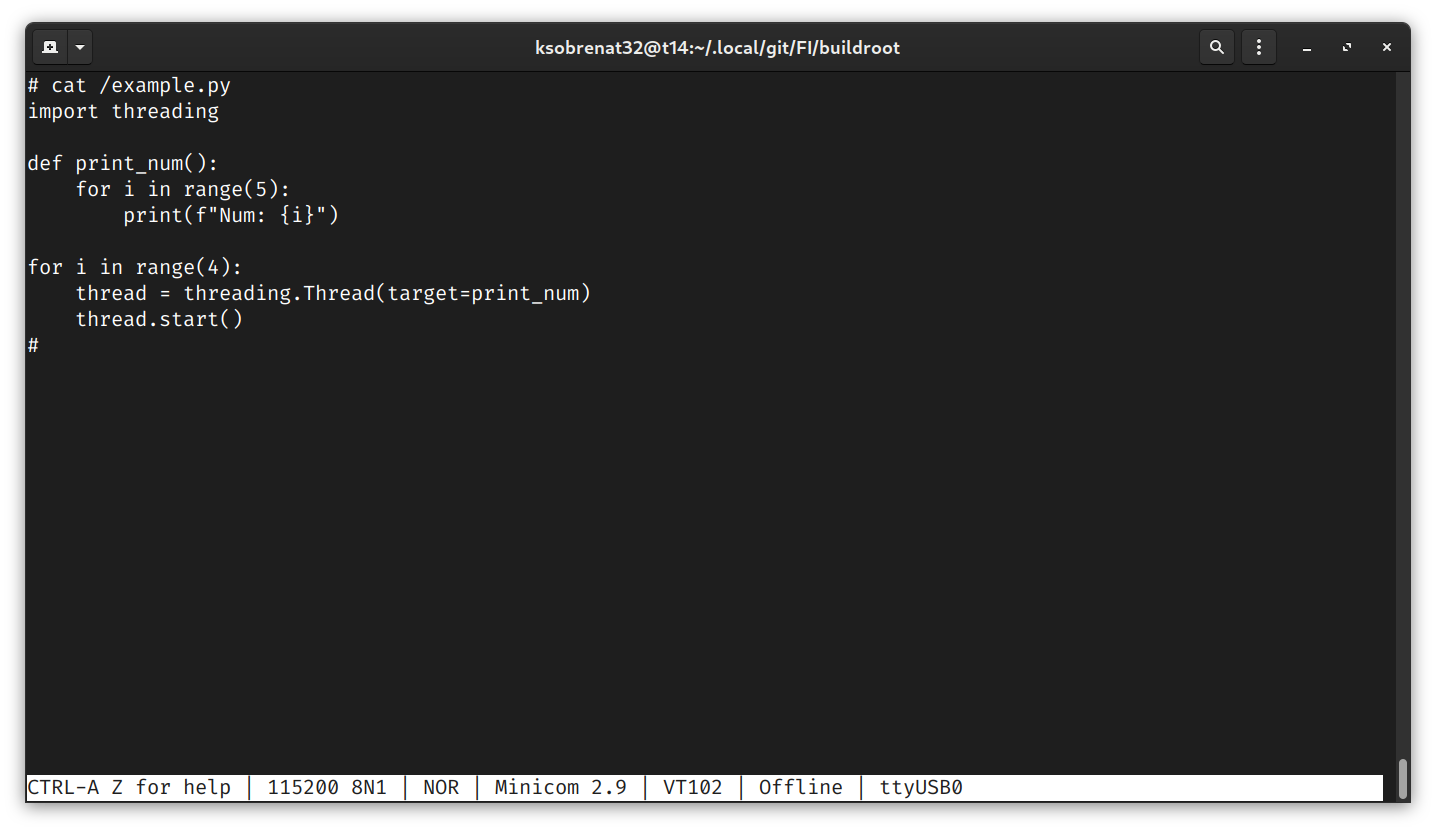
\includegraphics[width=\textwidth]{img/run-example-03}
			\caption{Ejemplo de código en python}
			\label{fig:boot}
		\end{center}
	\end{figure}


	\begin{figure}[H]
		\centering
		\begin{center}
			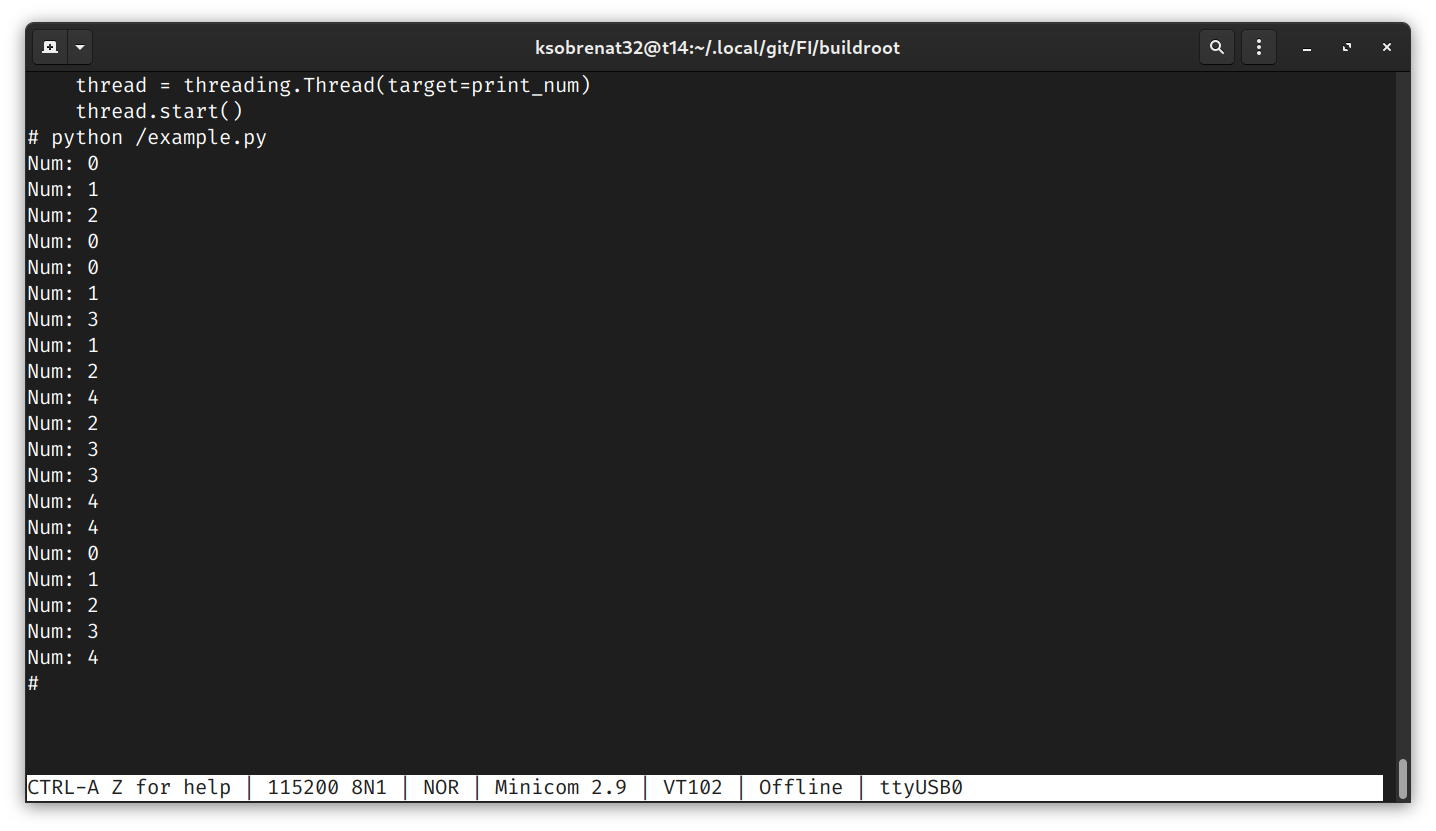
\includegraphics[width=\textwidth]{img/run-example-04}
			\caption{Ejecución de un script en python}
			\label{fig:boot}
		\end{center}
	\end{figure}


	\begin{figure}[H]
		\centering
		\begin{center}
			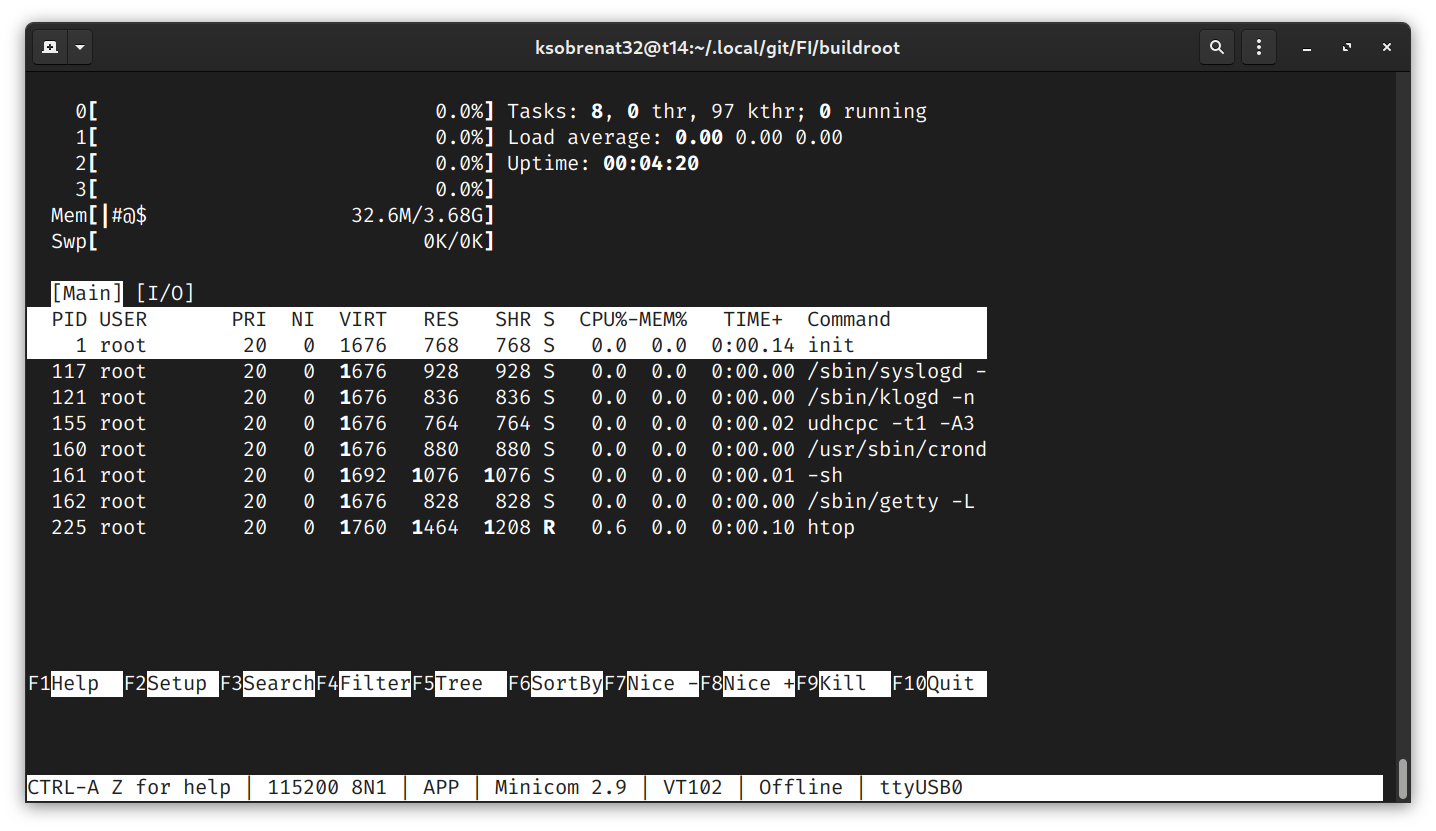
\includegraphics[width=\textwidth]{img/run-example-05}
			\caption{Uso de \texttt{htop} para monitorear el sistema}
			\label{fig:boot}
		\end{center}
	\end{figure}

	\section{Bibliografía}

	\begin{biblio}
		%for: https://www.ceupe.com/blog/sistema-embebido.html
		\item Administrador CEUPE. (s. f). \textit{Sistema embebido: Qué es, características y componentes}. Recuperado de: \textcolor{blue}{\underline{\url{https://www.ceupe.com/blog/sistema-embebido.html}}}
		%for: https://reboundeu.com/es/insights/blog/embedded-systems-explained-15/
		\item Rebound Electronics.  (s. f.). \textit{Explicación de los sistemas embebidos}. Recuperado de: \textcolor{blue}{\underline{\url{https://reboundeu.com/es/insights/blog/embedded-systems-explained-15/}}}
		%for: https://www.redhat.com/es/topics/linux/what-is-linux
		\item Red Hat. (2023, enero 3), \textit{Definición de Linux}. Recuperado de: \newline \textcolor{blue}{\underline{\url{https://www.redhat.com/es/topics/linux/what-is-linux}}}
		%for: https://trbl-services.eu/blog-linux-embebido-que-es/
		\item TRBL Services. (2021, julio 27), \textit{LINUX Embebido | Qué es, cómo funciona y para qué se usa}. Recuperado de: \newline \textcolor{blue}{\underline{\url{https://trbl-services.eu/blog-linux-embebido-que-es/}}}
		%for: https://buildroot.org/downloads/manual/manual.html
		\item Buildroot. (s. f.). \textit{Buildroot manual}. Recuperado de: \newline \textcolor{blue}{\underline{\url{https://buildroot.org/downloads/manual/manual.html}}}
		%for: https://www.ionos.mx/digitalguide/servidores/know-how/que-es-el-kernel/
		\item Equipo editorial de IONOS. (2021, julio 5). Kernel - El núcleo del sistema operativo. REcuperado de: \newline \textcolor{blue}{\underline{\url{https://www.ionos.mx/digitalguide/servidores/know-how/que-es-el-kernel/}}}
	\end{biblio}

\end{document}